\documentclass[aps,prx,twocolumn,superscriptaddress,nofootinbib,floatfix]{revtex4-2}

\usepackage{amsmath,amssymb,mathtools,bm}
\usepackage{booktabs}
\usepackage{graphicx}
\usepackage{microtype}
\usepackage[colorlinks=true,urlcolor=blue,linkcolor=blue,citecolor=blue]{hyperref}

\DeclareMathOperator{\diag}{diag}
\newcommand{\dd}{\mathrm{d}}
\newcommand{\ii}{\mathrm{i}}
\newcommand{\tr}{\operatorname{tr}}
\newcommand{\code}[1]{\texttt{#1}}

\begin{document}

\title{Trajectory-Resolved Modular Charge Response: A Finite-Size CPU Pilot}
\author{Asadullah Bhuiyan}
\affiliation{Department of Physics, Cornell University, Ithaca, New York 14853, USA}
\date{August 26, 2026}

\begin{abstract}
We analyze saved trajectory covariance histories of hard and soft programmable domain
walls using two state-resolved probes: a retarded charge response under modular-time
evolution and a static modular susceptibility.  The $20\times20$ histories contain ten
independent trajectories, and every nonlinear modular construction is performed before
averaging translated cuts or trajectories.  The hard wall exhibits endpoint-selective,
oppositely directed response on its two physical interfaces.  A finite-window Fourier
transform resolves mirror-related branches with $\omega\simeq b+v_{\rm F}|k|$ and
$v_{\rm F}\simeq0.28$ in opposite momentum sectors.  One soft-wall branch has the same
slope, while its partner is unresolved.  The small longitudinal window, nonzero and
damping-sensitive intercept, and strong aperture replicas make this an estimator pilot,
not a controlled conformal-dispersion measurement.
\end{abstract}

\maketitle

\section{Data and estimator order}

The two legacy histories use $N_x=N_y=20$, $n_{\rm shell}=1$, perfect correction,
$\alpha_1=1$, $\alpha_2=30$, raster-$y$ serial order, and a maximally mixed initializer.
The hard protocol has \code{dw\_truncation=true} and
\code{meas\_slab\_only=true}; the soft protocol has both controls false at execution.
Each history contains $S=10$ independent trajectories and every covariance from cycle
$0$ through 40.  We analyze cycles $21,25,29,33,37,40$ and all 20 translated
half-cylinders
\begin{equation}
 A(y_0)=[0,N_x)\times[y_0,y_0+N_y/2),\qquad y_0=0,\ldots,19.
\end{equation}
For every observable we first evaluate the nonlinear estimator for each cut, average the
20 cuts within a trajectory, and only then form trajectory means and percentile-bootstrap
intervals.  Translated cuts and checkpoints are never treated as independent samples.

\section{Gaussian modular response}

The repository stores the centered covariance $G_A$, so the restricted correlation
matrix is
\begin{equation}
 C_A=\frac{\mathbf{1}_A+G_A}{2}
    =U\diag(\nu_a)U^\dagger .
\end{equation}
For the Gaussian reduced density operator
\begin{equation}
 \hat\rho_A=Z_A^{-1}\exp\!\left[-\sum_{ij}(h_A)_{ij}
 \hat c_i^\dagger\hat c_j\right],
\end{equation}
the one-body modular Hamiltonian is
\begin{equation}
 \begin{aligned}
 h_A&=\log\frac{\mathbf{1}_A-C_A}{C_A}
 =U\diag(\varepsilon_a)U^\dagger,\\
 \varepsilon_a&=\log\frac{1-\nu_a}{\nu_a}.
 \end{aligned}
\end{equation}
We clip occupations to $[\epsilon,1-\epsilon]$, with primary
$\epsilon=10^{-10}$ and controls $10^{-8},10^{-12}$.

\subsection{Retarded response}

Let $P_0$ project onto both local orbitals of the perturbed unit cell.  The many-body
charge-phase kick $e^{-\ii\lambda\hat N_0}$ induces the correlation-matrix tangent
\begin{equation}
 X(0)=-\ii[P_0,C_A].
\end{equation}
Since $[h_A,C_A]=0$, modular-time evolution gives
\begin{equation}
 X(\tau)=e^{-\ii h_A\tau}X(0)e^{\ii h_A\tau},\qquad
 \chi^R(\boldsymbol r,\tau)=\tr[P_{\boldsymbol r}X(\tau)].
 \label{eq:retarded}
\end{equation}
In the modular eigenbasis,
\begin{equation}
 \widetilde X_{ab}(\tau)=-\ii(\nu_b-\nu_a)(\widetilde P_0)_{ab}
 e^{-\ii(\varepsilon_a-\varepsilon_b)\tau}.
\end{equation}
The spatial sum of Eq.~\eqref{eq:retarded} vanishes.  We therefore use the signed wall
dipole rather than a normalized center of mass,
\begin{equation}
 M_y(\tau)=\sum_{\substack{x:\,d(x,x_w)\leq2\\y_{\rm rel}}}
 (y_{\rm rel}-y_{\rm src})\chi^R(x,y_{\rm rel},\tau).
\end{equation}
The early-time slope $v$ is fitted over $0.1\leq\tau\leq0.8$.

\subsection{Static susceptibility}

For $h_\lambda=h_A-\lambda P_0$ and $f(x)=(1+e^x)^{-1}$, the exact Fr\'echet
derivative is
\begin{equation}
 (\delta C_A)_{ab}=-f^{[1]}(\varepsilon_a,\varepsilon_b)
 (\widetilde P_0)_{ab},
\end{equation}
where
\begin{equation}
 f^{[1]}(x,y)=
 \begin{cases}
 [f(x)-f(y)]/(x-y),&x\neq y,\\
 -f(x)[1-f(x)],&x=y.
 \end{cases}
\end{equation}
The local static susceptibility is
$\chi^{\rm stat}(\boldsymbol r)=\tr[P_{\boldsymbol r}\delta C_A]$.
Positive $\lambda$ lowers the local modular chemical potential and attracts charge.

\begin{figure*}[t]
 \centering
 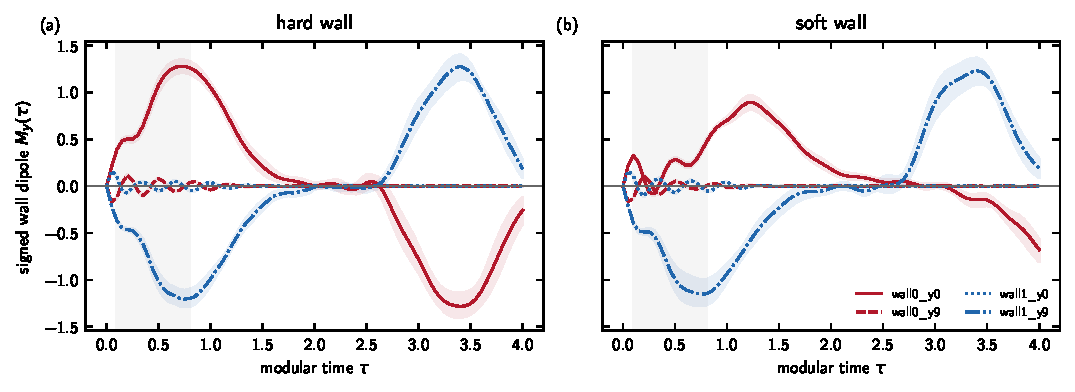
\includegraphics[width=0.96\textwidth]{figures/retarded_modular_dipoles.pdf}
 \caption{Trajectory-resolved signed wall dipoles at cycle 40 for the hard and soft
 wall protocols.  Curves are means over $S=10$ independent maximally-mixed-initialized
 trajectories after averaging the 20 translated cuts within each trajectory; bands are
 trajectory-bootstrap 95\% intervals.  The shaded interval is the slope-fit window
 $0.1\leq\tau\leq0.8$.  One endpoint on each physical wall carries the dominant response,
 with opposite signs between wall orientations.}
 \label{fig:dipoles}
\end{figure*}

\section{Real-space response}

At cycle 40 the active source slopes are
\begin{align}
 (v_{0},v_{1})_{\rm hard}&=(1.514,-1.417),\\
 (v_{0},v_{1})_{\rm soft}&=(0.384,-1.286),
\end{align}
where $0$ denotes $(x,y_{\rm rel})=(5,0)$ and $1$ denotes $(15,9)$.  The
complementary endpoints are at least an order of magnitude weaker.  As an exploratory
orientation-aligned summary, define
\begin{equation}
 H=\frac{v_0-v_1}{2}.
\end{equation}
Trajectory bootstraps with 5000 resamples give
\begin{align}
 H_{\rm hard}&=1.466\ [1.350,1.575],\\
 H_{\rm soft}&=0.835\ [0.715,0.943],\\
 H_{\rm hard}-H_{\rm soft}&=0.630\ [0.474,0.795].
\end{align}
The endpoint pair entering $H$ was selected after inspecting all four source responses;
accordingly, $H$ is a descriptive handedness score, not a prespecified hypothesis test or
quantized transport coefficient.

The static response is strongly local.  Its source-averaged integrated value is 0.1352
for the hard wall and 0.1259 for the soft wall, while transverse leakage is of order
$10^{-3}$.  It acts here as a local modular-compressibility diagnostic, not a chirality
estimator.  The maximum retarded total-charge residual is $1.04\times10^{-15}$.
Analytic retarded and static responses agree with centered finite differences at relative
errors $1.67\times10^{-9}$ and $1.43\times10^{-9}$, respectively.

\section{Finite-window Fourier response}

Projecting Eq.~\eqref{eq:retarded} onto the five-column wall window gives
$\chi_w(y,\tau)$.  We compute
\begin{equation}
 \chi_w(k,\omega)=\Delta\tau\sum_{j,y}
 e^{\ii\omega\tau_j}e^{-\ii k(y-y_{\rm src})}
 w(\tau_j)e^{-\eta\tau_j}\chi_w(y,\tau_j),
 \label{eq:fourier}
\end{equation}
with a Tukey taper, primary damping $\eta=0.35$, ten independent momenta
$k_n=2\pi n/10$, and $0\leq\tau\leq4$.  Because the half-cylinder is open along
$y_{\rm rel}$, Eq.~\eqref{eq:fourier} is a source-resolved finite-window transform rather
than a momentum-conserving susceptibility.

For each wall orientation, we select its low-frequency momentum sector: $k<0$ for
$(5,0)$ and $k>0$ for $(15,9)$.  At the four nonzero points with
$0<|k|\leq2.6$, the largest $|\chi_w|$ peak in $0.2\leq\omega\leq2.5$ is fitted to
\begin{equation}
 \omega_{\rm peak}=b+v_{\rm F}|k|.
\end{equation}
A branch is rejected when at least half of its peaks remain on the lower frequency-search
boundary.

\begin{figure*}[t]
 \centering
 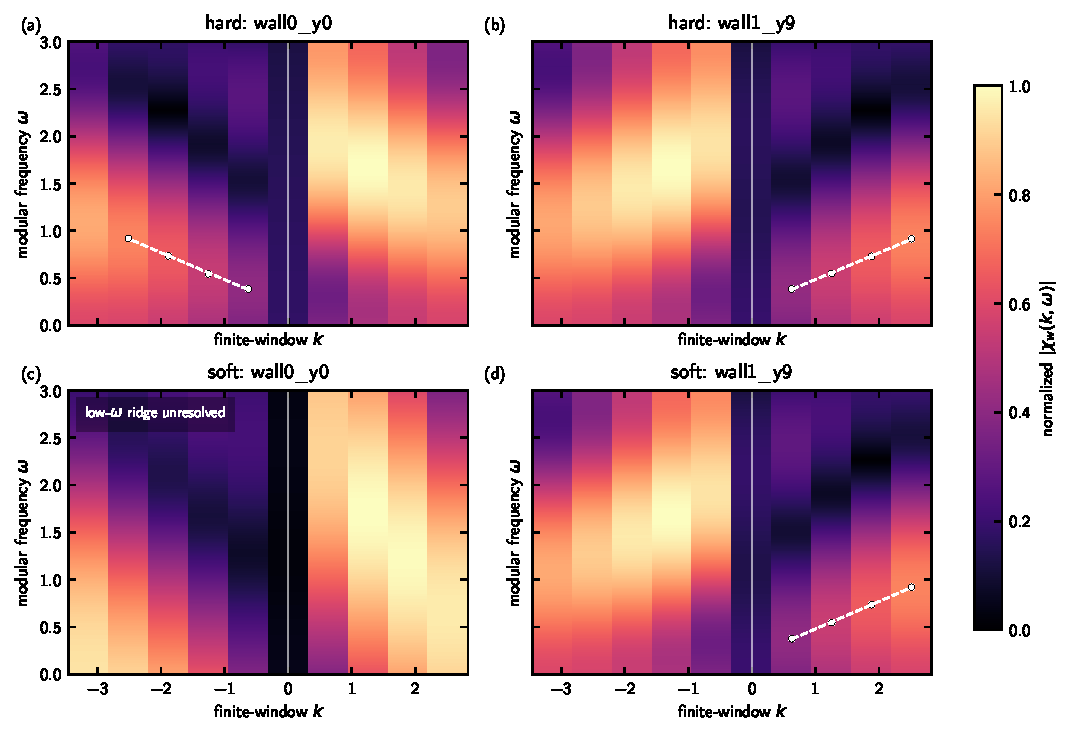
\includegraphics[width=0.96\textwidth]{figures/finite_window_modular_fourier_spectra.pdf}
 \caption{Normalized finite-window Fourier magnitude at cycle 40.  The four independent
 low-frequency ridge points and linear fits are overlaid where the branch passes the
 boundary check.  The hard-wall branches occupy opposite momentum sectors and are mirror
 related.  The soft $(15,9)$ branch is resolved, whereas the soft $(5,0)$ response piles
 up at the low-frequency search boundary.  Every panel is formed per trajectory before
 averaging $S=10$ trajectories.}
 \label{fig:fourier}
\end{figure*}

\begin{table}[b]
\caption{Crude Fourier-ridge fits at cycle 40.  Intervals are trajectory-bootstrap 95\%
intervals.  The $\eta$ range reports fits at $\eta=0.20,0.35,0.50$.}
\label{tab:ridge}
\begin{ruledtabular}
\begin{tabular}{lccc}
branch & $v_{\rm F}$ & ensemble $R^2$ & $\eta$ range\\
\hline
hard $(5,0)$ & $0.279\,[0.270,0.290]$ & 0.999 & 0.266--0.318\\
hard $(15,9)$ & $0.282\,[0.274,0.291]$ & 0.999 & 0.267--0.309\\
soft $(5,0)$ & unresolved & --- & ---\\
soft $(15,9)$ & $0.284\,[0.277,0.294]$ & 0.999 & 0.271--0.321\\
\end{tabular}
\end{ruledtabular}
\end{table}

The resolved branches share $v_{\rm F}\simeq0.28$ and the hard-wall pair appears in
opposite physical momentum sectors.  This is consistent with a linear chiral modular
branch.  It is not yet a controlled $\omega=v k$ result: only four momenta enter each fit,
the primary intercept is $b\simeq0.19$--$0.20$, $b$ moves strongly with damping, and
finite-aperture replicas are prominent in Fig.~\ref{fig:fourier}.  In particular, the soft
wall does not yield a clean two-interface dispersion at this size.

\section{Scope and reproducibility}

This pilot validates the response estimators and motivates a larger-$N_y$ study, but it
does not establish a conformal velocity, central charge, level, or manuscript gate.  The
ten trajectories use a maximally mixed initializer and are not a substitute for the
redesigned random-pure W1 ensemble.  The executed notebook, raw response arrays, Fourier
product, summary tables, and figures are stored together under
\path{notebooks/modular_response_cpu_pilot/}.  The source covariance archives remain
immutable and are addressed by SHA-256 digest in the notebook manifest.

\end{document}
